\atividade{Atividade 3.2.2 – Implantar e reabilitar sistemas coletivos de abastecimento de água no meio rural e as soluções de saneamento associadas}

\textbf{Correspondência:} Acordo de Empréstimo, Parte 3.2(b); nota técnica: NT IAT – Subcomponente 3.2.b (IAT, 2026b); NT 2026 – Componente 3, Saneamento Rural (IAT, 2026a).

\textbf{Valor da atividade:} R\$~250,15 milhões (empréstimo BIRD: R\$~183,00 milhões; contrapartida: R\$~67,15 milhões).

\textbf{Ações:} 3.2.2.1 Implantação dos modelos de gestão; 3.2.2.2 Trabalho técnico-social; 3.2.2.3 Implantação e reabilitação dos sistemas coletivos de abastecimento de água; 3.2.2.4 Programa Sanepar Rural; 3.2.2.5 Esgotamento sanitário nas comunidades atendidas com água; 3.2.2.6 Esgotamento sanitário em propriedades de mananciais (área da SEAB); 3.2.2.7 Supervisão e gerenciamento das obras.

A atividade compreende a implantação e a reabilitação de sistemas coletivos de abastecimento de água em comunidades rurais, as soluções de esgotamento sanitário associadas e os modelos de gestão responsáveis pela prestação dos serviços após as obras. O objetivo comum às ações é ampliar o acesso sustentável aos serviços de abastecimento de água e de esgotamento sanitário no meio rural do Paraná, no período de 2027 a 2033 (IAT, 2026a; IAT, 2026b). As metas físicas compreendem 83 sistemas coletivos implantados pelo IAT, 222 sistemas do Programa Sanepar Rural e soluções individuais de esgotamento sanitário em 6.367 domicílios.

As ações articulam-se em sequência (Figura~\ref{articulacao}). Os modelos de gestão e o trabalho técnico-social antecedem as obras: formalizam a adesão dos municípios, caracterizam as famílias e as condições sanitárias de cada comunidade e estruturam a entidade gestora de cada sistema. Na sequência, o IAT implanta os sistemas de abastecimento de água e as soluções de esgotamento sanitário, com supervisão independente das obras, e a Sanepar executa o Programa Sanepar Rural com recursos de contrapartida.

\begin{figure}[H]
  \centering
  \caption{Articulação das ações de abastecimento de água e esgotamento sanitário rural}\label{articulacao}
  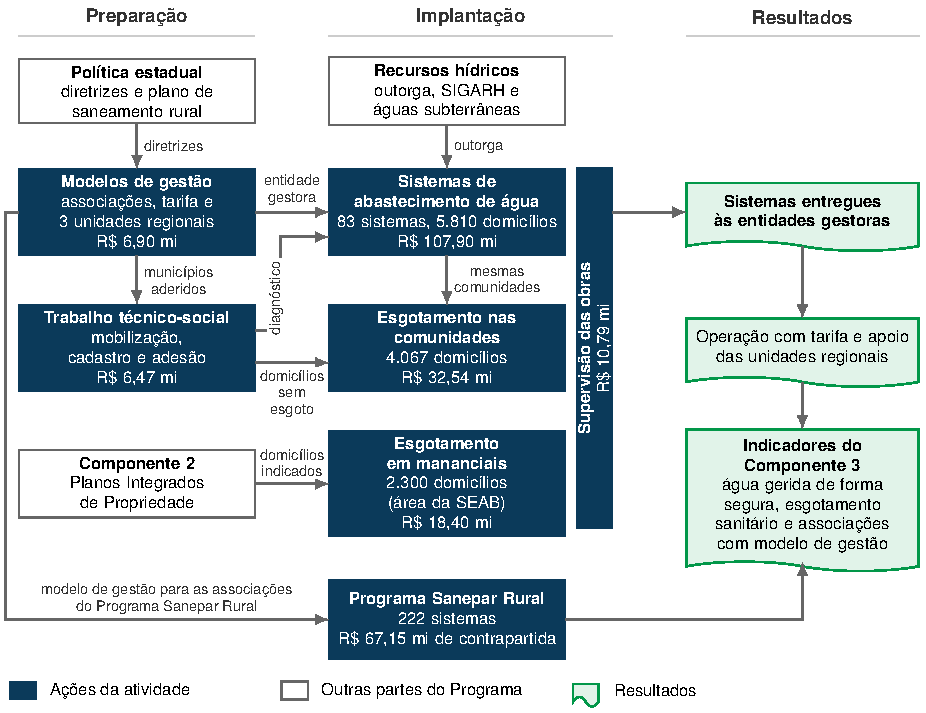
\includegraphics[width=15.68cm]{figuras/f-articulacao.pdf}
  \fonteMOP{Fonte: IAT (2026), com valores da planilha PSH\_CUSTO\_Consolidada (PARANÁ, 2026).}
  % Texto alternativo: Diagrama da articulação entre as sete ações da atividade, da preparação social e institucional à entrega dos sistemas e aos indicadores do componente.
\end{figure}

A Figura~\ref{crono-atividade} apresenta o período de execução e o investimento anual de cada ação.

\begin{figure}[H]
  \centering
  \caption{Período de execução e investimento anual das ações de abastecimento de água e esgotamento sanitário rural (R\$~milhões)}\label{crono-atividade}
  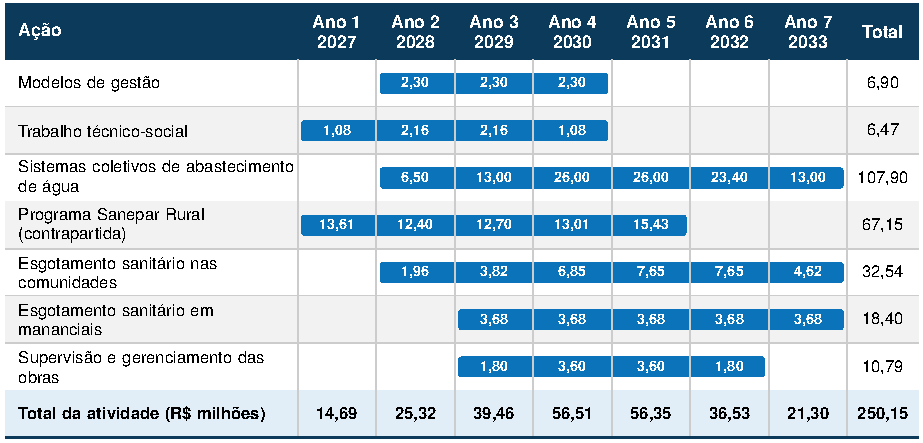
\includegraphics[width=15.64cm]{figuras/g-crono-atividade.pdf}
  \fonteMOP{Fonte: Planilha PSH\_CUSTO\_Consolidada, versão v2408 (PARANÁ, 2026). Valores arredondados; o total anual corresponde à soma dos valores exatos da planilha.}
  % Texto alternativo: Cronograma de 2027 a 2033 com o investimento anual de cada ação e o total da atividade por ano.
\end{figure}
